\subsection{Loss functions}
The problem of decoy quality assessment is essentially a ranking problem: we have to arrange decoys according to 
the proximity to the corresponding native structure, which is quantified using GDT-TS score. \tchanged{The ranking algorithms 
was previously applied to the problem of model quality assessment \cite{jing2016sorting}, and also 
used along with neural networks to rank image descriptions \cite{gong2013deep}.}

During the training procedure we load several decoy structures of one target (minibatch) into memory, compute the 
output of the network and the average loss:
$$ L = \frac{1}{N^{2}_B} \sum_{i=1,j=1, i \neq j}^{N_B} L_{ij} $$ 
where $N_B$ is the number of decoys in a minibatch. Afterwards, we compute the gradient of the average loss with respect 
to the network parameters and update them using Adam algorithm.

We used the margin ranking loss for each pair of decoys. Let a decoy representation be denoted as $x_i$ and therefore the output
of the network on this decoy will be $f(x_i)$. Next, let $y_{ij}$ be the ordering coefficient of the two decoys we pick:
$$
y_{ij} = \begin{cases}
               1& \text{GDT-TS}_i \leq \text{GDT-TS}_j \\
               -1& \text{GDT-TS}_i > \text{GDT-TS}_j \\
            \end{cases}
$$
Here $\text{GDT-TS}_i$ is the GDT-TS score of the $i$-th decoy. In principle, any target function can be chosen. 
The pairwise ranking scoring function has the following expression:

$$ L_{ij} = w_{ij} \cdot \max \left[ 0, 1 - y_{ij} \left( f \left( x_i \right) - f \left( x_j \right) \right) \right] $$

the term $w_{ij}$ represents an example weight:

$$
w_{ij} = \begin{cases}
               1& \left| \text{GDT-TS}_i - \text{GDT-TS}_j \right| > T \\
               0& \text{otherwise} \\ 
            \end{cases}
$$

where the $T$ is a threshold constant set to 0.1{\AA}. If the two decoys are too similar, 
we avoid scoring them against each other during the training. 



\subsection{Evaluation criteria}
\tchanged{
We evaluated our algorithm using the correlation coefficients and loss criterions. The correlation coefficents 
were computed between the score of our model and GDT-TS metric for all the decoys of each target protein in a test set and then averaged.
}
The loss criterion is the deviation of the GDT-TS of the best decoys for a protein from the GDT-TS score of the decoy with the lowest score:
$$ 
Loss = | max_i( \text{GDT-TS}_i ) - \text{GDT-TS}_{argmin_i(f(x_i))} |
$$ 

\subsection{Optimization and dataset sampling}
The optimization procedure of deep convolutional networks usually is stochastic: the function value and gradient 
is estimated on a small subset (batch) of all the training 
examples. We used the batch of size 10 due to the memory limitations. Afterward the parameters of the model are 
changed in the direction of the estimated gradient.
The parameter update step was performed using the Adam algorithm \cite{kingma2014adam}. 

The dataset was sampled in the following way: first we chose a random protein from the dataset, then we sample decoys of this protein. 
The procedure is repeated for all the 
proteins in a dataset. One pass through all the proteins in a dataset is called epoch. 
The decoys are sampled in a homogeneous way: we divide all the decoys into $M$ clusters by the value of GDT-TS score. 
Precisely, the decoy $i$ belongs to the cluster  
number $ \left[ \frac{\max(\text{GDT-TS}) - \text{GDT-TS}_i}{\max(\text{GDT-TS}) - \min(\text{GDT-TS})} \right] + 1$, 
where $\max(\text{GDT-TS})$ and $\min(\text{GDT-TS})$ are computed for all the decoys of 
the chosen protein. If there are empty clusters, then we take secon decoys from each non-empty and so on until we filled the batch. 
At the end of each epoch we randomly shuffle the order of protein and the order of decoys in each cluster. 

Each decoy from the selected batch is randomly rotated and translated. The rotations are sampled uniformly \cite{shoemake1992uniform}. 
The translation are chosen in such a way, that the bounding box of the translated protein lies within the box of the size 120x120x120\AA. 

To select the final model we randomly divided the training set into training and validation subsets. The validation subset consists of 
35 targets and their decoys. This subset was not sampled during the training. 
Figure \ref{Fig:TrainingLoss} shows the Kendal tau, Pearsor R coefficients and the loss on the vaidation subset. 
The final model was chosen according to the minimum loss (epoch 40).
\begin{figure}[H]
    \centering
    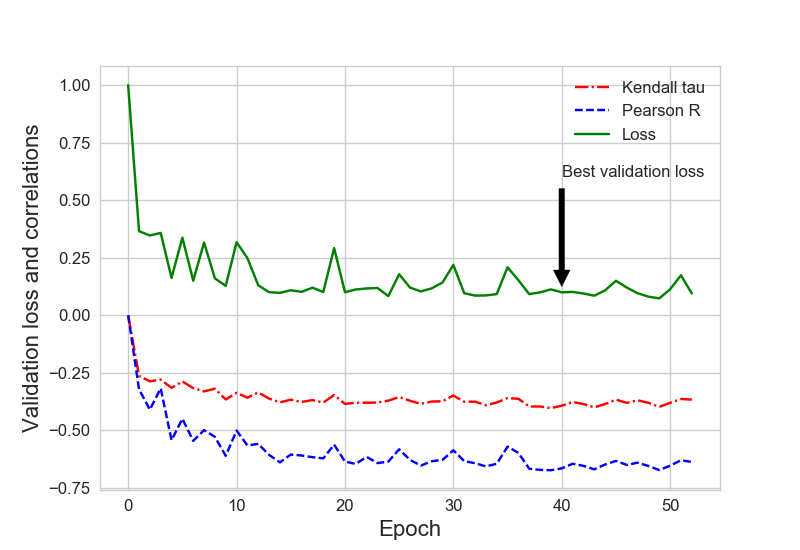
\includegraphics[width=\linewidth]{Fig/kendall_validation.png}
    \caption{The loss, Kendal tau and Pearson R coefficients evaluated on the validation subset during the training procedure. The epoch 
    denotes that all the targets in the training subset were sampled.}
    \label{Fig:TrainingLoss}
\end{figure}

The table \ref{Tbl:TrainingResults} summarizes the performance metrics on the training and validation sets for the model at epoch 40.

\begin{table}[H]
\begin{center}
\begin{tabular}{ c | c | c | c | c }
    Data subset & Loss & Pearson & Spearmann & Kendall \\
    \hline
    Training set     &0.146 &0.71 &0.61 &0.45 \\
    Validation set   &0.135 &0.71 &0.59 &0.44 \\ \hline

\end{tabular}
  \caption {Results of the model from epoch 40 on the training and validation subsets.}
    \label{Tbl:TrainingResults}
\end{center}
\end{table}